% !TeX TS-program = LuaLatex
% !TeX spellcheck = en
% !BIB TS-program = biber
% !TeX encoding = UTF-8 Unicode
% -*- coding: UTF-8; -*-
% vim: set fenc=utf-8
%%%%%%%%%%%%%%%%%%%%%%%%%%%%%%%%%%%%%%%%%%%%%%%%%%%%%%%%%%%%%%%%%%%%%
% il y a aussi tikzposter qui est bien cf https://www.overleaf.com/learn/latex/Posters
\documentclass[landscape,a0]{a0poster}
%\documentclass[landscape,a0, draft]{a0poster}
%%%%%%%%%%%%%%%%%%%%%%%%%%%%%%%%%%%%%%%%%%%%%%%%%%%%%%%%%%%%%%%%%%%%%
\newcommand{\doc}{poster}

\newcommand{\Title}{
Learning heterogeneous delays of spiking neurons for motion detection
%Learning hetero-synaptic delays for motion detection in a population of Spiking Neurons
%FAST MOTION DETECTION USING HETERO-SYNAPTIC DELAYS IN A LAYER OF SPIKING NEURONS
}
\newcommand{\AuthorAG}{Antoine Grimaldi}
\newcommand{\AuthorCB}{Camille Besnainou}
\newcommand{\AuthorHL}{Hugo Ladret}
\newcommand{\AuthorLP}{Laurent U Perrinet}
\newcommand{\EmailLP}{laurent.perrinet@univ-amu.fr}
\newcommand{\EmailAG}{antoine.grimaldi@univ-amu.fr}
\newcommand{\EmailHL}{hugo.ladret@univ-amu.fr}
\newcommand{\orcidLP}{0000-0002-9536-010X}
\newcommand{\orcidHL}{0000-0001-7999-3751}
\newcommand{\orcidAG}{0000-0002-3107-4788}
\newcommand{\Address}{Institut de Neurosciences de la Timone (UMR 7289); Aix Marseille Univ, CNRS; Marseille, France}%
\newcommand{\Affiliation}{Aix Marseille Univ, CNRS}%
\newcommand{\CityLP}{Marseille, France}%
\newcommand{\WebsiteLP}{https://laurentperrinet.github.io}%
\newcommand{\Abstract}{
\begin{itemize}
\item In a recent review paper, we reported experimental evidence for the presence of precise spiking motifs embedded in recordings from biological neural tissues and neuromorphic data~\cite{grimaldi_precise_2023}. 

\item Inspired by this neuroscientific observation, we develop a model for the efficient detection of temporal spiking motifs based on a layer of spiking neurons with heterogeneous synaptic delays.

\item We show that this can be formalized as a time-invariant logistic regression that can be trained on labeled data. We demonstrate its application to synthetic naturalistic videos transformed into event streams similar to the output of the retina or to event-based cameras and for which we will characterize the accuracy of the model in detecting visual motion.
\end{itemize}
%The response of a biological neuron depends on the precise timing of afferent spikes. This temporal aspect of the neural code is essential to understand information processing in neurobiology and applies particularly well to the output of neuromorphic hardware such as event-based cameras. However, most artificial neural models do not take advantage of this important temporal dimension of the neural code. Inspired by this neuroscientific observation, we develop a model for the efficient detection of temporal spiking motifs based on a layer of spiking neurons with heterogeneous synaptic delays. The model uses the property that the diversity of synaptic delays on the dendritic tree allows for the synchronization of specific arrangements of synaptic inputs as they reach the basal dendritic tree. We show that this can be formalized as a time-invariant logistic regression that can be trained on labeled data. We demonstrate its application to synthetic naturalistic videos transformed into event streams similar to the output of the retina or to event-based cameras and for which we will characterize the accuracy of the model in detecting visual motion. In particular, we quantify how the accuracy can vary as a function of the overall computational load showing it is still efficient at very low workloads. This end-to-end, event-driven computational building block could improve the performance of future spiking neural network (SNN) algorithms and in particular their implementation in neuromorphic chips.
}
\newcommand{\Keywords}{time code, event-based computations, spiking neural networks, motion detection, efficient coding, logistic regression
}
\newcommand{\Acknowledgments}{AG and LP received funding from the European Union ERA-NET CHIST-ERA 2018 research and innovation program under grant agreement N° ANR-19-CHR3-0008-03 (``\href{http://aprovis3d.eu/}{APROVIS3D}''). LP received funding from the ANR project  N° ANR-20-CE23-0021 (''\href{https://laurentperrinet.github.io/grant/anr-anr/}{AgileNeuroBot}''). %HL received funding from a University of Montreal Artificial Intelligence scholarship. For the purpose of open access, the author has applied a CC BY public copyright licence to any Author Accepted Manuscript version arising from this submission.
}
\newcommand{\presynaddr}{a} % pre address
\newcommand{\postsynaddr}{b} % post address
\newcommand{\numevent}{N_{ev}} % total number of events
\newcommand{\presynaddrspace}{\mathcal{A}} %presynaptic address space
\newcommand{\postsynaddrspace}{\mathcal{B}} %postsynaptic address space
\newcommand{\Npol}{N_\text{p}} % number of polarity
\newcommand{\Nneuron}{N_\text{n}} % number of output neurons in the layer
\newcommand{\arank}{r} % address index
\newcommand{\bias}{b} % bias for the MLR model
\newcommand{\synapse}{\mathcal{S}} % synapse
\newcommand{\synapticweight}{w} % synaptic weight
\newcommand{\synapticdelay}{\delta} % synaptic delay
\newcommand{\ranksyn}{s} % synapse index
\newcommand{\Nsyn}{N_{s}} % total number of synapses
\newcommand{\activeweights}{\mathcal{W}}
\newcommand{\timev}{t} % time
\newcommand{\polev}{p} % polarity
\newcommand{\event}{\epsilon} % event
\newcommand{\eventstream}{\xi} % stream of events
\newcommand{\TS}{S} % time surface
\newcommand{\neuron}{\mathbf{n}} % neuron in the SNN (defined by the spatial position and the channel)
\newcommand{\postneuron}{\mathbf{m}} % post synaptic neuron in the SNN (defined by the spatial position and the kernel)
\newcommand{\channel}{\mathbf{p}} % channel
\newcommand{\layer}{\mathbf{L}} % layer
\newcommand{\ms}{\si{\milli\second}}%
\newcommand{\us}{\si{\micro\second}}%
\newcommand{\timecontext}{T} % time context (cf HOTS) matrice gathering last event times
\newcommand{\current}{I} % post synaptic current
\newcommand{\volt}{u} % membrane potential
\newcommand{\volts}{V} % matrix of membrane potentials
\newcommand{\gain}{\gamma} % homeostatic gain
\newcommand{\simil}{\beta} % similarity value
\newcommand{\Nclass}{N_\text{class}} % number of classes for MLR:
\newcommand{\Nx}{N_\text{X}}
\newcommand{\Ny}{N_\text{Y}}
\newcommand{\Ntime}{N_\text{t}}
\newcommand{\kernel}{K} % convolution kernel
%\newcommand{\kernelind}{\mathbf{k}} % indice of the kernel
\newcommand{\kernelind}{k} % indice of the kernel
\newcommand{\Kx}{K_\text{x}}
\newcommand{\Ky}{K_\text{y}}
\newcommand{\Ktime}{K_\text{t}}
\newcommand{\classiflayer}{\mathbf{C}}
\newcommand{\class}{c} % class k of the MLR
\newcommand{\lrweights}{\theta} % matrix of MLR weights
\newcommand{\lrtrue}{y} % true value of the prediction for MLR
\newcommand{\loss}{J} % cost function for MLR
\newcommand{\softmax}{\sigma}
\newcommand{\actfreq}{f}
\newcommand{\decision}{\hat{y}}
\newcommand{\speed}{v}
\newcommand{\Nspeed}{N_v}
%
\newcommand{\colorsec}{red}
\newcommand{\colorsubsec}{gray}
%%%%%%%%%%%%%%%%%%%%%%%%%%%%%%%%%%%%%%%%%%%%%%%%%%%%%%%%%%%%%%%%%%%%%
\usepackage{fontspec}
\usepackage{titlesec}
\titleformat*{\section}{\huge\bfseries}
\usepackage{float} %allows me to use [H] with figures to insert figures in multicol env (poster)
\usepackage{graphicx}
\usepackage{amsmath}
\usepackage{amssymb}
\usepackage{hyperref}
\usepackage{multicol}
\usepackage[utf8]{inputenc}
\defaultfontfeatures{Mapping=tex-text,Scale=MatchLowercase}
\setmainfont{Alegreya}
\DeclareMathOperator*{\argmax}{arg\,max}
\usepackage[
%style=chem-acs,
style=numeric,						% numeric style for reference list
citestyle=numeric-comp,
%style=alphabetic-verb,
giveninits=false,
maxbibnames=1,
%firstinits=true,
%style=apa,
%maxcitenames=1,
%maxnames=3,
%minnames=1,
%maxbibnames=99,
dateabbrev=true,
giveninits=true,
%uniquename=init,
url=false,
doi=false,
isbn=false,
eprint=false,
texencoding=utf8,
bibencoding=utf8,
autocite=superscript,
backend=biber,
%sorting=none,
sorting=none,
sortcites=false,
%articletitle=false
]{biblatex}%

\bibliography{FastMotionDetection.bib}

%%%%%%%%%%%%%%%%%%%%%%%%%%%%%%%%%%%%%%%%%%%%%%%%%%%%%%%%%%%%%%%%%%%%%
\columnsep=2cm % This is the amount of white space between the columns in the poster
\columnseprule=2pt % This is the thickness of the black line between the columns in the poster
\def\columnseprulecolor{\color{black}}
\usepackage{multirow}
%%%%%%%%%%%%%%%%%%%%%%%%%%%%%%%%%%%%%%%%%%%%%%%%%%%%%%%%%%%%%%%%%%%%%
%\sffamily
\usepackage[most]{tcolorbox}
\newtcbox{\mybox}{size = normal, on line}% boxsep=3mm,
%outer arc=1mm, arc=3mm,
%boxrule=2mm,colback=red!10!white, colframe=red!50!black, arc is angular}
\begin{document}
%----------------------------------------------------------------------------------------
%	POSTER HEADER
%----------------------------------------------------------------------------------------
% The header is divided into two boxes:
% The first is 75% wide and houses the title, subtitle, names, university/organization and contact information
% The second is 25% wide and houses a logo for your university/organization or a photo of you
% The widths of these boxes can be easily edited to accommodate your content as you see fit
\vspace*{-2cm}
%
\begin{minipage}[b]{0.175\textwidth}
%\hspace*{2cm}

\includegraphics[width=.4\textwidth]{figures/int_logo.pdf}

\includegraphics[width=.6\textwidth]{figures/amu_logo.pdf}\\
%\vspace{-.5cm}
\begin{center}
\color{blue}
\Large
\href{mailto://\EmailAG}{\EmailAG} \hspace{.2cm}
\end{center}
\vspace{1cm}
\end{minipage}
%
\begin{minipage}[b]{.65\textwidth}
\begin{center}
\VeryHuge
\textbf{\color{\colorsec}
\Title
} \\ % \color{Black}
\end{center}
\large
\centering \hspace{.5cm} \textbf{
\AuthorAG , \hspace{.1cm}
%\AuthorCB , \hspace{.1cm}
%\AuthorHL  \hspace{.1cm}
\& \hspace{.1cm}
\AuthorLP
%\hspace{.5cm}
 -
%
\large
%\hspace{.1cm}
\Address} \\
%\vspace{1cm}
\end{minipage}
%
\begin{minipage}[t]{0.175\textwidth}
%
%\vskip{-8cm}
\vspace{-9cm}
%\begin{tabular} {c c}
%
\includegraphics[height=.20\textwidth]{figures/cnrs_logo.pdf} & \includegraphics[height=.20\textwidth]{figures/brain-logo-240.jpg} \\
%\multicolumn{2}{c}{
\includegraphics[height=.15\textwidth]{figures/chistera_logo.pdf}}\\
%\end{tabular}

\includegraphics[height=.2\textwidth]{figures/cnrs_logo.pdf}\hspace{1cm} 
\includegraphics[height=.2\textwidth]{figures/chistera_logo.pdf}\hspace{1cm}
%\includegraphics[height=.15\textwidth]{figures/brain-logo-240.jpg}
%\vskip{-2cm}
%\hspace*{5cm}
%
\includegraphics[height=.15\textwidth]{figures/chistera_logo.pdf}\\
%\vspace*{3cm}
%\hspace{3cm}
%
\includegraphics[height=.20\textwidth]{figures/cnrs_logo.pdf}
%\hspace{1cm}
%\includegraphics[height=.20\textwidth]{figures/brain-logo-240.jpg}
%\\
\vspace{.25cm}

\begin{center}
\color{blue}
\Large
\href{https://laurentperrinet.github.io/publication/grimaldi-22-bc/}{https://laurentperrinet.github.io
\\ /publication/grimaldi-22-bc/} \end{center}
\vspace{2cm}

\end{minipage}
%
\vspace*{-1.5cm}
\hrule
\vspace{5pt}
\hrule
%----------------------------------------------------------------------------------------
\begin{multicols}{3} % This is how many columns your poster will be broken into, a portrait poster is generally split into 2 columns
%----------------------------------------------------------------------------------------
%	ABSTRACT
%----------------------------------------------------------------------------------------
\section*{\color{\colorsec}Abstract \vspace{.3cm}  \hrule}
\vspace{-2.5cm}
\Abstract
%----------------------------------------------------------------------------------------
%	MLR
%----------------------------------------------------------------------------------------
\section*{\color{\colorsec}Heterogeneous delays model (HD-SNN)\hrule}
%
\vspace*{-2.5cm}
\subsection*{\color{\colorsubsec}Illustration}
%
\begin{figure}[H]
    \centering
    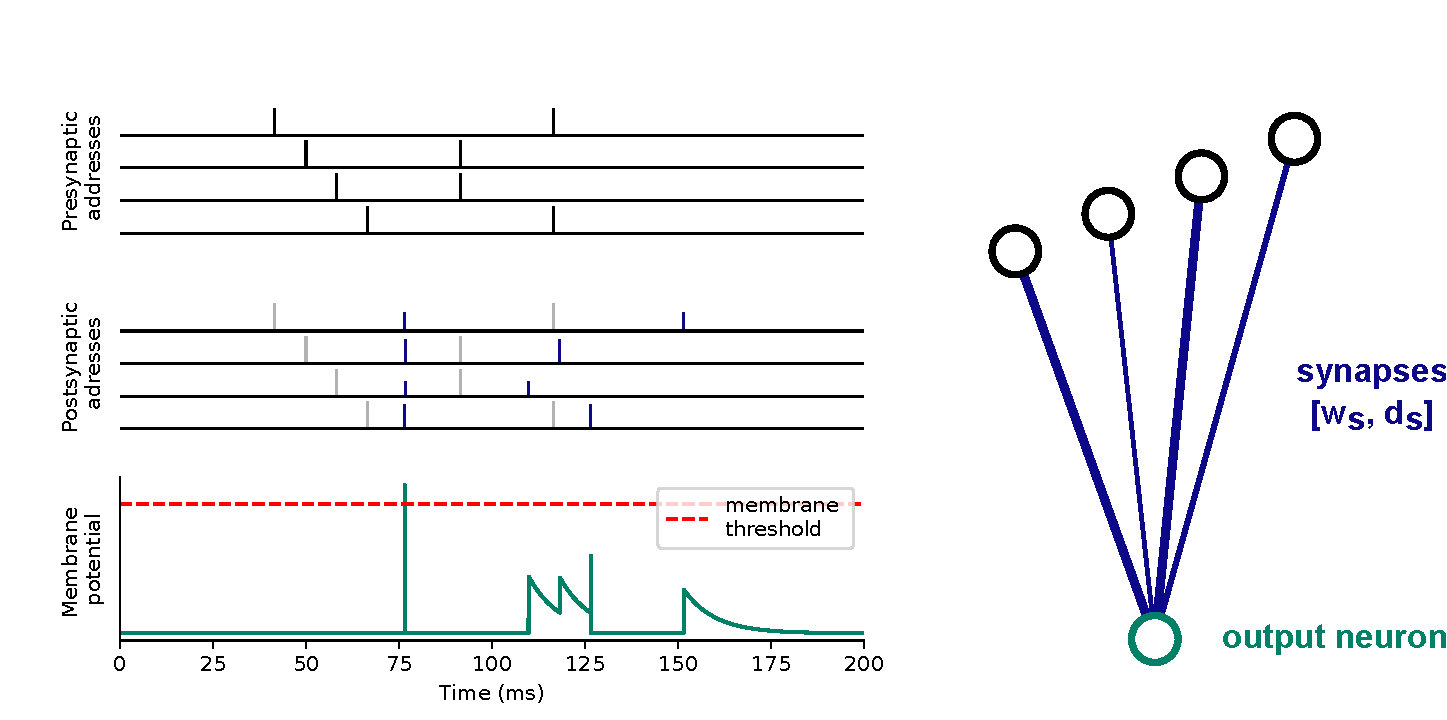
\includegraphics[width=0.980\linewidth]{figures/HDSNN_graph.pdf}
    \caption{\textbf{The core mechanism of the HD-SNN model.} \textit{(Top-Left)}~Two spiking motifs are emitted from four presynaptic neurons. Once integrated by the synapses of the postsynaptic neuron~\textit{(Right)}, the spiking motifs are shifted in time by the synaptic delays and weighted by the synaptic weights~\textit{(Middle-Left)}. When they reach the soma of the postsynaptic neuron, the different spikes contribute to a modification of its membrane potential according to an activation function. In this example, we use the same activation function as for a Leaky Integrate and Fire neuron~\textit{(Bottom-Left)}. The first spiking motif is synchronized by the synaptic delays and causes a sudden rise in the membrane potential of the postsynaptic neuron. An output spike is emitted when the membrane potential reaches the threshold and it is then reset.   \textit{(Right)}~An illustration of a spiking neuron with different synaptic weights (represented by the thickness of the synapses) and different synaptic delays (represented by the length of the synapses). }%
    \label{fig:izhikevich}%
\end{figure}
%TODO: changer le temps d'occurence des spikes
%\vspace*{1.5cm}
\subsection*{\color{\colorsubsec}Mathematical formalism}
%
\textbf{Event stream:}
%The spikes reaching our SNN can be formalized as:
$$
\mybox{$\event = \{(\presynaddr_\arank, 1, \timev_\arank)\}_{\arank \in [1,\numevent]}$}
$$
where $\numevent \in \mathbb{N} $ is the total number of events, $\timev_\arank$ is the time occurrence of event number $\arank$ and $\presynaddr_\arank$ an associated address , which is typically in the form $\presynaddr_\arank=(x_\arank, y_\arank, \polev_\arank)$. \\
%
\\
\textbf{Spiking neuron with hetero-synaptic delays:}
%
$$
\mybox{$\synapse = \{(\presynaddr_\ranksyn, \postsynaddr_\ranksyn, \synapticweight_\ranksyn, \synapticdelay_\ranksyn)\}_{\ranksyn \in [1,\Nsyn]}$}
$$
is a set of $\Nsyn$ synapses, where each synapse $\synapse_\ranksyn$ is associated to a presynaptic address $\presynaddr_\ranksyn$, a postsynaptic address $\postsynaddr_\ranksyn$, a weight $\synapticweight_\ranksyn$ and a delay $\synapticdelay_\ranksyn$. We can define the synapses of the receptive field of neuron $\postsynaddr$ as such: $\synapse^\postsynaddr =  \{(\presynaddr_\ranksyn, \postsynaddr_\ranksyn, \synapticweight_\ranksyn, \synapticdelay_\ranksyn) \| \postsynaddr_\ranksyn=\postsynaddr\}_{\ranksyn \in [1,\Nsyn]}  \subset \synapse$.
They transform the event stream as input into: 
$$
\mybox{$\event_\postsynaddr = \{(\presynaddr_\arank, \synapticweight_\arank, \timev_\arank+\synapticdelay_\ranksyn) \| \presynaddr_\arank = \presynaddr_\ranksyn \}_{\arank \in [1,\numevent], \ranksyn \in \synapse^\postsynaddr}$}
$$

%
\columnbreak
%
\noindent
\textbf{Temporal convolution:}

\noindent By discretizing time, we can transform any event-based input from an event-based camera into a Boolean matrix $A \in \{0, 1 \}^{\Npol \times \Ntime \times \Nx \times \Ny}$ where the ones define the events. Using this dense representation, the processing of $A$ by neuron $\postsynaddr$ can be written as: %
%
$$
\mybox{$\forall \timev, \; \;
\mathcal{C}_\postsynaddr(x_\postsynaddr, y_\postsynaddr, \timev)
= \sum_{p, \delta_x, \delta_y, \synapticdelay_\timev} \kernel_\postsynaddr(p, \delta_x, \delta_y, \synapticdelay_\timev) \cdot A(p, x - \delta_x, y - \delta_y, \timev-\synapticdelay_\timev)
$}
$$
%
where $\kernel_\postsynaddr$ gives the weights as a function of relative addresses, $\delta_x$ and $\delta_y$, and synaptic delays $\delta_\timev$.\\
%
\\
\textbf{Multinomial logistic regression (MLR):}

\noindent We can further assume that synaptic motifs should be similar across different positions, so we can define a spatio-temporal convolutional operator: $\mathcal{C}_\class = \kernel_\class \ast A$, where $\class$ combines different postsynaptic neurons sharing the same class. Then, the activation function of our model is a softmax function implementing a form of MLR, in analogy to a spiking Winner-Takes-All network~\cite{nessler_bayesian_2013}:
$$
\mybox{
$ \forall x, y, \timev, \forall \class \in [1, N_\class], \; \;
Pr(k=\class \; \vert \;  x, y, \timev) =
\frac {\exp  (\mathcal{C}_\class(x, y, \timev) +\bias_\class) }{Z(x, y, \timev)}
$
}
$$
%
\vspace{1cm}
%
\begin{figure}[H]
    \centering
    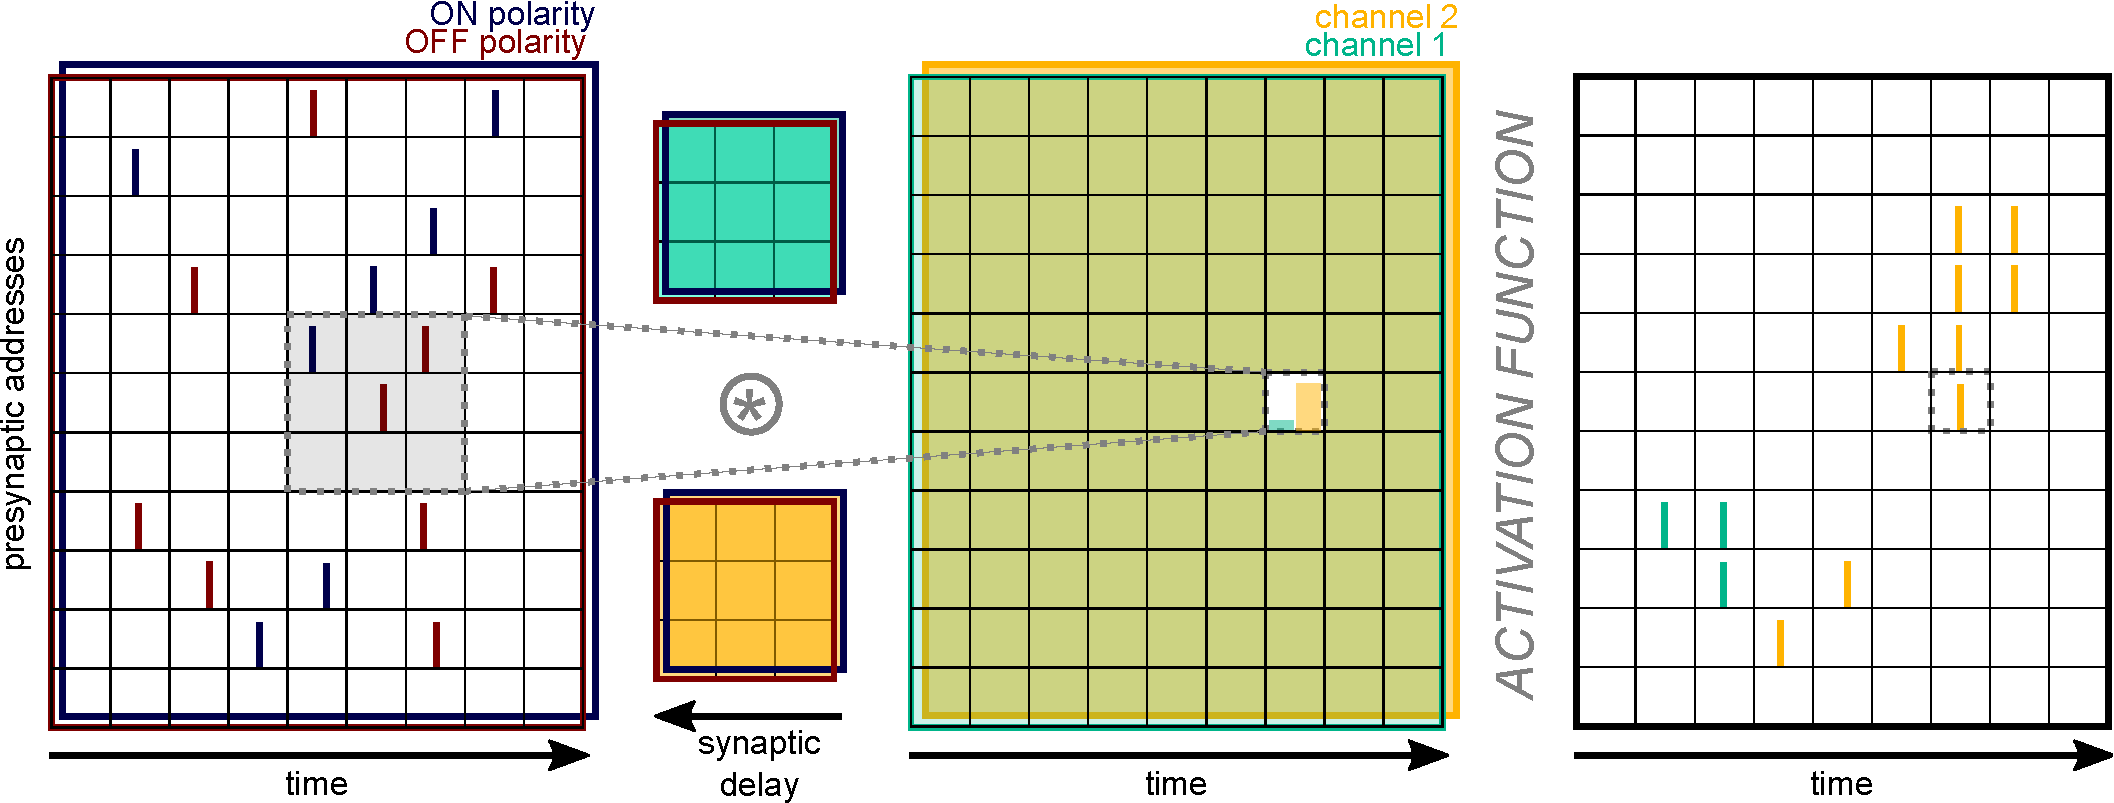
\includegraphics[width=\linewidth]{figures/HDSNN_conv.pdf}
    % 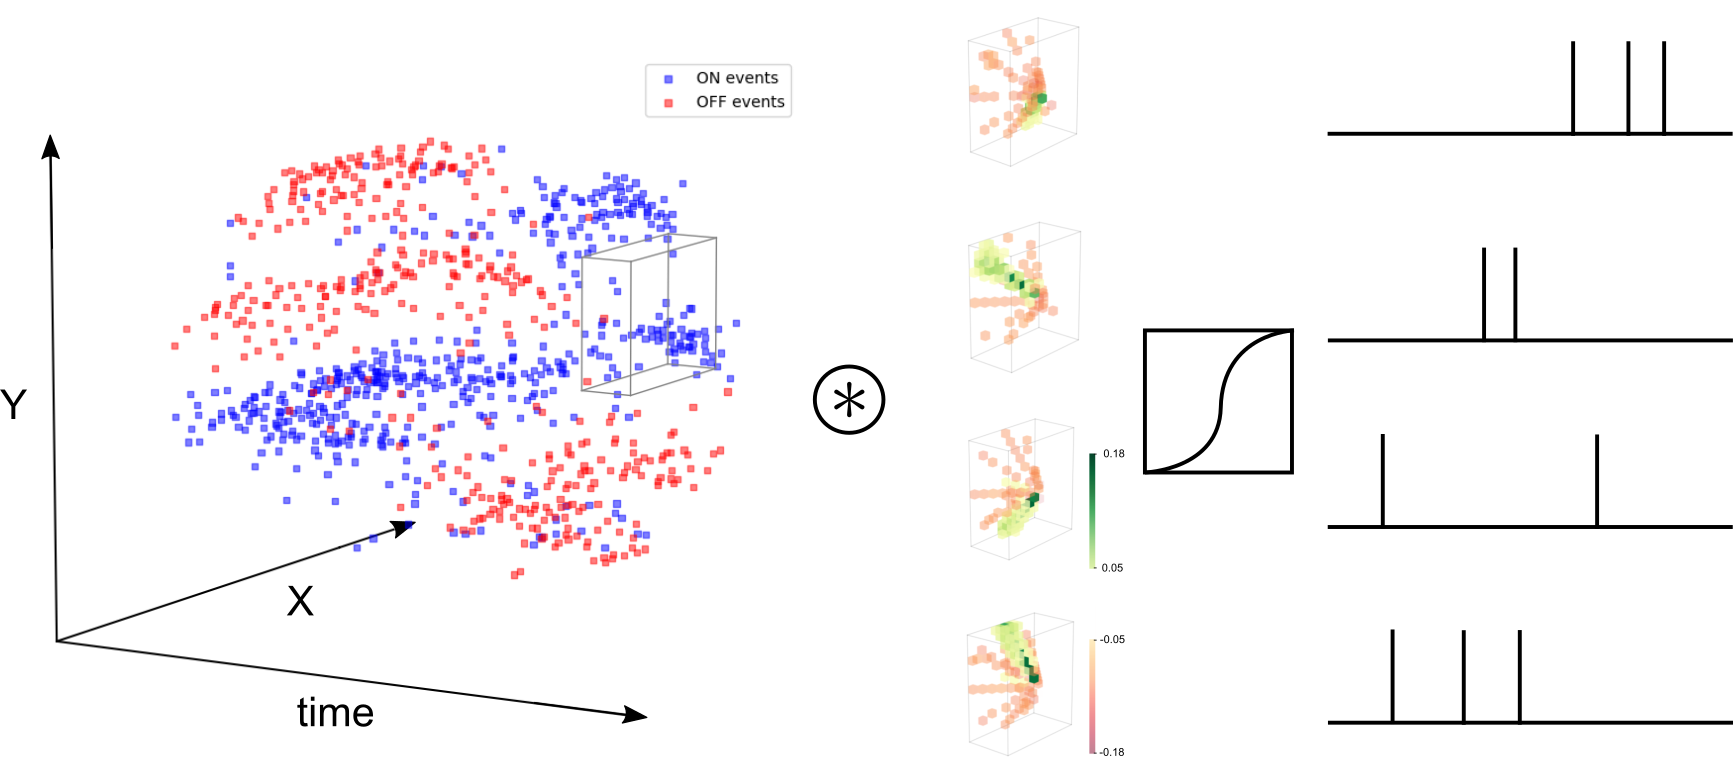
\includegraphics[width=\linewidth]{figures/HD-SNN.png}
    \caption{
    % \textbf{- HD-SNN illustration. From left to right:} A 3D representation of the event stream as output of the DVS. A 3D convolution is applied, on the dense representation of the input, along the $X$ and $Y$ spatial axes (defining the DVS pixel grid) and the temporal axis. There are as many kernels as the possible number of motion classes in the recording. For clarity, only $4$ kernels are illustrated and some weights are not represented in the voxel grid. For each voxel on the dense representation of the event stream as input, the output of the 3D convolution is processed by the non-linearity of the MLR model (i.e. softmax function). The output of the MLR gives a probability for each class, associated to a specific kernel, to emit an output event, or spike. With an appropriate spiking mechanism, here a winner-takes-all, we obtain, as output of the HD-SNN model, a new spike train with the different spikes associated to a specific motion class. }
    \textbf{Applying HD-SNN to the motion detection task.} \textit{(Left)}~We plot here a 2D representation of the input event stream. A spatio-temporal convolution is applied to the dense representation of the input with $2$ distinct convolutional kernels (the green and orange kernels) that will define the output channels (if you have two axes $X$ and $Y$ to represent the presynaptic addresses as for the pixel grid of a DVS, you obtain a 3D convolution). \textit{(Middle)}~The output of the convolution is processed by the nonlinearity of the MLR model (i.e., the softmax function). \textit{(Right)}~By adding a spiking mechanism, we obtain a new spike train with the spikes associated to the different motion classes.}
    \label{fig:model}
\end{figure}
%----------------------------------------------------------------------------------------
%	MOTION CLOUDS
%----------------------------------------------------------------------------------------
\section*{\color{\colorsec}Event-based input \vspace{.2cm}  \hrule}
%
\vspace{-1cm}
%
\begin{figure}[H]
    \centering
    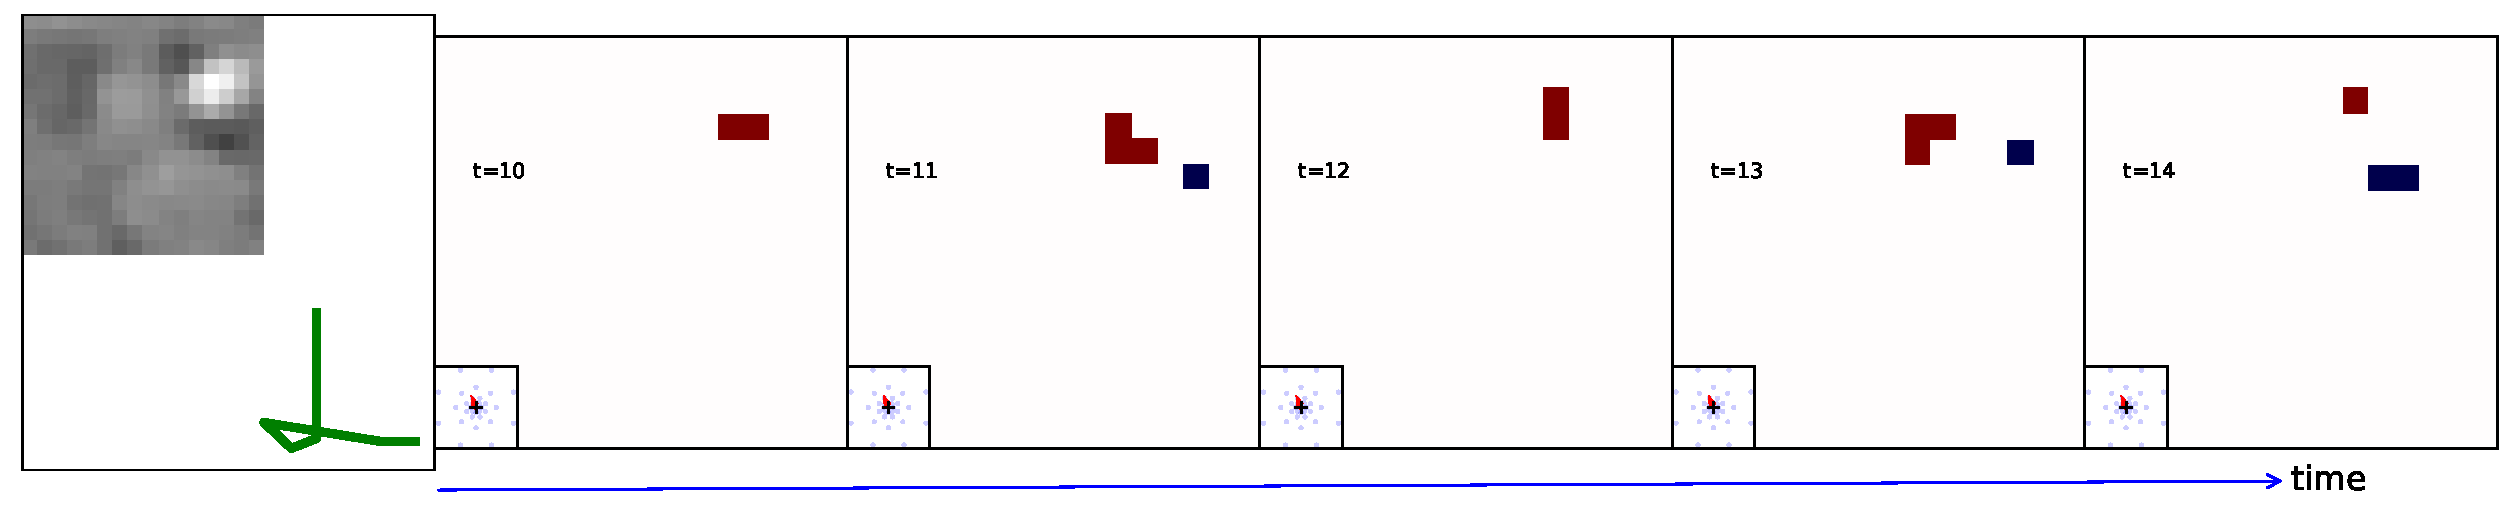
\includegraphics[width=0.95\linewidth]{figures/motion_task.pdf}
    \caption{
        {\bf - Motion Detection Task.} \textit{(Left)}~We use large natural images ($256\times256$) in which an aperture ($64\times64$) extracts a cropped image around the view axis. To mimic the effect of a saccadic eye movement, the view axis moves according to a stepwise random walk. We show such a trajectory with a length of $128$ time steps (green line). \textit{(Right)}~Snapshots of the synthetic event stream at different time steps. The dynamics of the cropped image translated according to the trajectory as a function of time produces a naturalistic movie, which is then transformed into an event-based representation. Mimicking the retina, this representation encodes proportional increases or decreases in luminance, i.e. ON (red) and OFF (blue) events, in each pixel of the image. In the lower left corner of the snapshots, the translation vector is shown in red as one of the possible classes of motion.}
    \label{fig:motion_task}
\end{figure}
%
%\vspace{1cm}
\columnbreak
%
%----------------------------------------------------------------------------------------
%	RESULTS
%----------------------------------------------------------------------------------------
\section*{\color{\colorsec}Results \vspace{.2cm}\hrule}
% ------------------------------------------------------
\vspace{-2.5cm}
\subsection*{\color{\colorsubsec}Learning heterogeneous delays}
%
\vspace{-1cm}
\begin{figure}[H]
    \centering
    %\vspace{-3cm}
    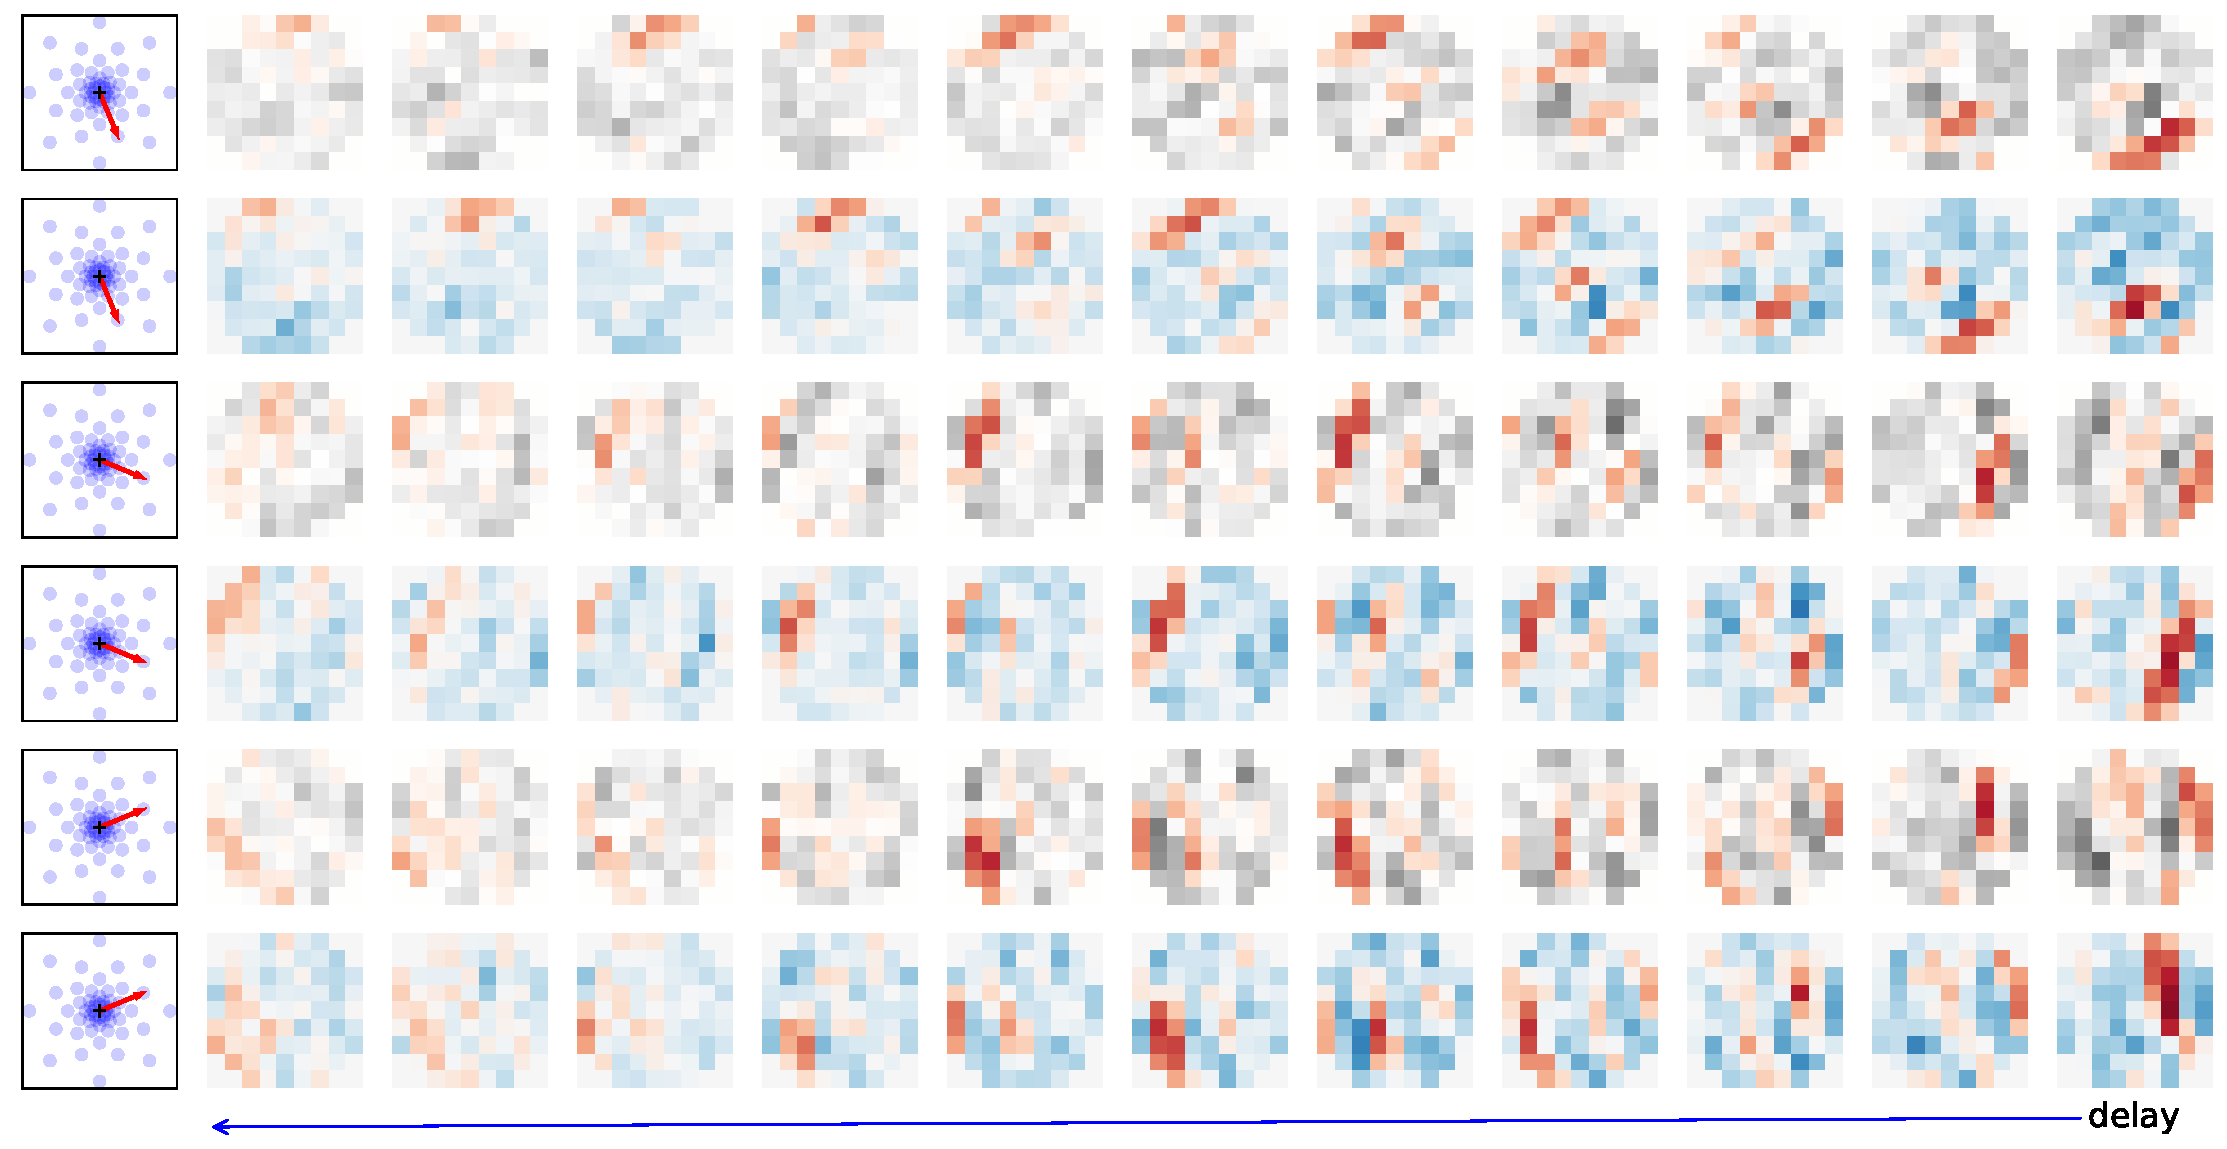
\includegraphics[width=.8\linewidth]{figures/motion_kernels.pdf}
    %\vspace{-.5cm}
    \caption{
    	\textbf{Representation of the weights} for $8$ directions for one speed (among the $8 \times 3$ different kernels of the model) as learned on the dataset of naturalistic scenes. Directions are shown as red arrows on the left. The spatio-temporal kernels are represented as slices of spatial weights at different delays. Due to the observed symmetry between the ON and OFF event streams, we report that the kernels for the OFF polarities are very similar and are not shown here. Different kernels are selective to the different motion directions and we observe for all kernels an orientation preference perpendicular to the orientation. 
%      % These weights are associated to a specific delay on the \textit{delays} axis and to a presynaptic address defined on the two other axes. %	For the sake of clarity, the values in range $[-0.05, 0.05]$ are not shown.    One sees positive (excitatory) coefficients for the specific direction of motion but also negative (inhibitory) coefficients for other directions.
	}
    \label{fig:kernels}
\end{figure} 
% ------------------------------------------------------
\subsection*{\color{\colorsubsec}Accuracy as a function of the number of computations}
% ------------------------------------------------------
\begin{figure}[H]
    \centering
    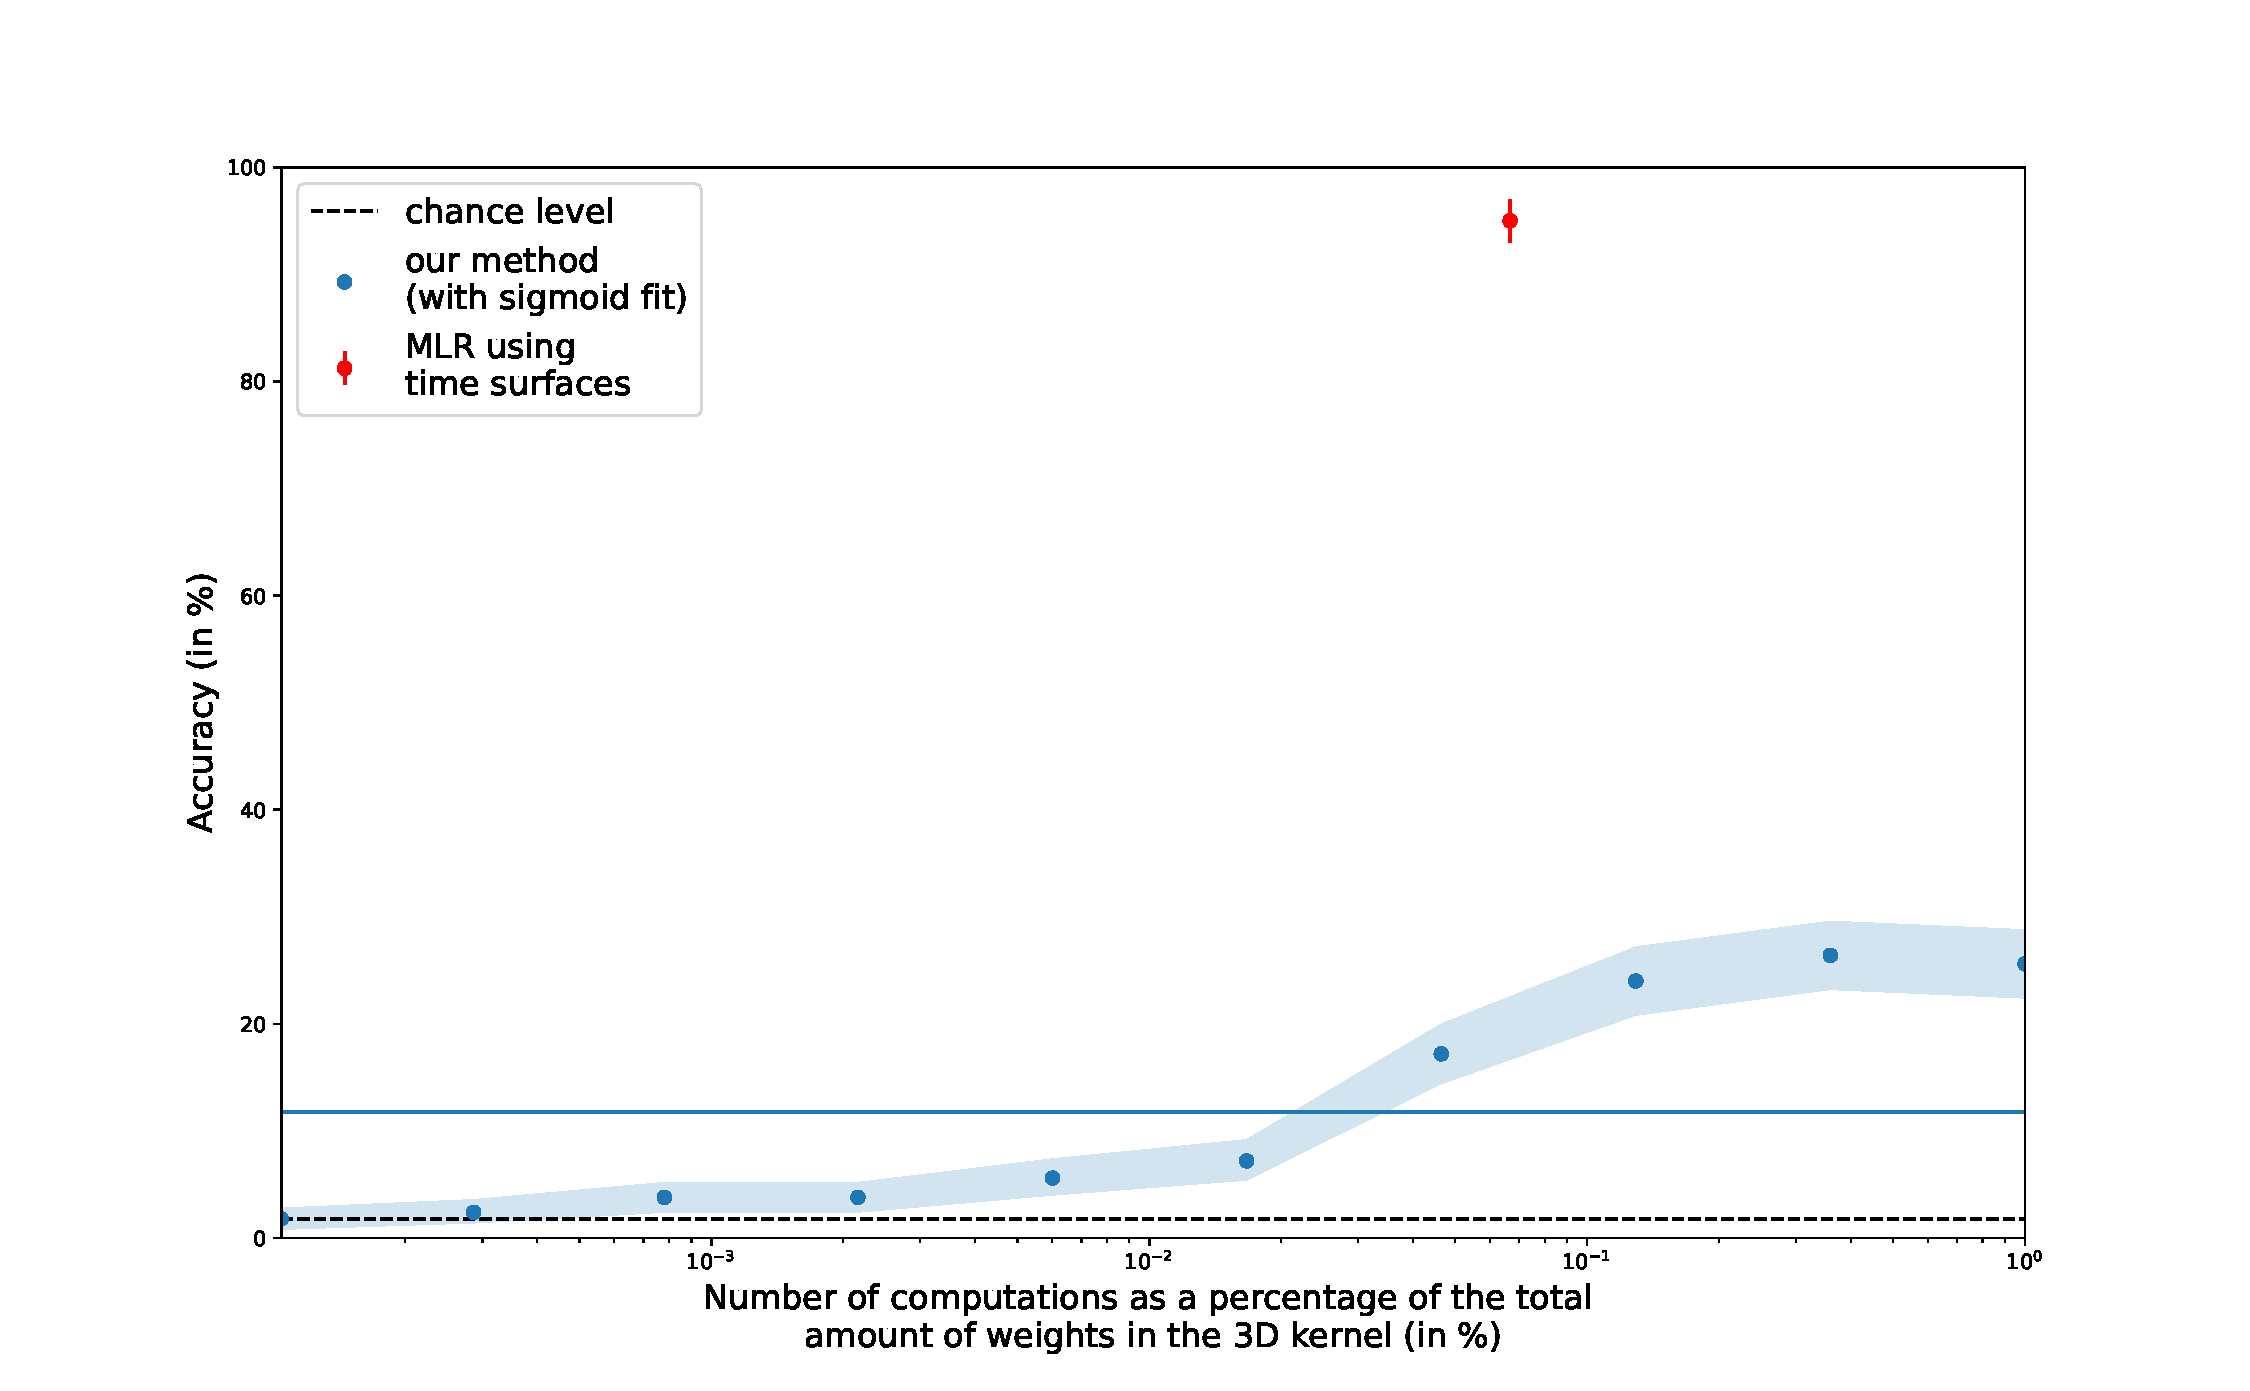
\includegraphics[width=0.6\linewidth]{figures/quant_accuracy.pdf}
    \caption{\textbf{Accuracy as a function of computational load} for the HD-SNN model (blue dots) with error bars indicating the 5\% - 95\% quantiles and a sigmoid fit (blue line). The relative computational load (on a logarithmic axis) is controlled by changing the percentage of nonzero weights relative to the dense convolution kernel. As we prune the coefficients, we observe a stable accuracy value, with a drop observed at about 25 times fewer computations.}
    \label{fig:accuracy}
\end{figure}
%----------------------------------------------------------------------------------------
%	CONCLUSIONS
%----------------------------------------------------------------------------------------
%\section*{\color{\colorsec}Conclusion \vspace{.2cm} \hrule}
%\vspace{-2.5cm}
%
%We have introduced a generic SNN using hetero-synaptic delays and shown how it compares favorably with a state-of-the-art event-based algorithm used for classification~\cite{lagorce_hots_2017}. This shows that we may use the precise timing of a spike to enhance neural computations.
%
%One advantage of our model is the generality of the approach.
%Indeed, this supervised learning scheme can be extended to a novel task by defining a new set of supervision pairs (for instance supervised by local orientation) which would lead to the emergence of new kernels adapted to this new task.
%This constitutes a major advantage over other algorithms which derive event-based algorithms from specific physical rules. %(see for instance~\cite{Benosman12} for computing the optic flow using the luminance conservation rule).
%We aim at extending the application of this model on more generic datasets acquired in natural conditions for progressively more complex tasks such as time-to-contact maps, but also to neurophysiological data.
%
\vspace{1cm}
\hrule
%	REFERENCES
%----------------------------------------------------------------------------------------
%\vspace{-1cm}
\printbibliography
%----------------------------------------------------------------------------------------
%----------------------------------------------------------------------------------------
%	ACKNOWLEDGEMENTS
%----------------------------------------------------------------------------------------
%\hrule
%\vspace{-1cm}
\section*{Acknowledgments}
\vspace{-1cm}
\Acknowledgments
%----------------------------------------------------------------------------------------
%\renewcommand*{\bibfont}{\normalfont\fontsize{20}{12}\selectfont}
%
%\printbibliography
\end{multicols}
%
\end{document}
